\section{Specifications}

To be able to participate to the race, our car needed to validate some technical specifications. \textbf{Groupe Sigma} gave us a set of rules to follow.

\subsection{Technical Specifications}
To enter the race, the car have to:
\begin{itemize}
\item have 4 wheels without any other ground support
\item be 30x25x25cm\footnote{Lenght$\cdot$Width$\cdot$Height} maximum
\item weight 4kg maximum
\item have a maximal total battery power of 7800mAh 
\item be equiped with 2 motors maximum
\item be equiped with a circuit-cutter in case of emergency
\item be autonomously controlable with the use of captors such as cameras, lidars, ultra-sound\dots
\end{itemize}

\begin{figure}[!h]
\centering
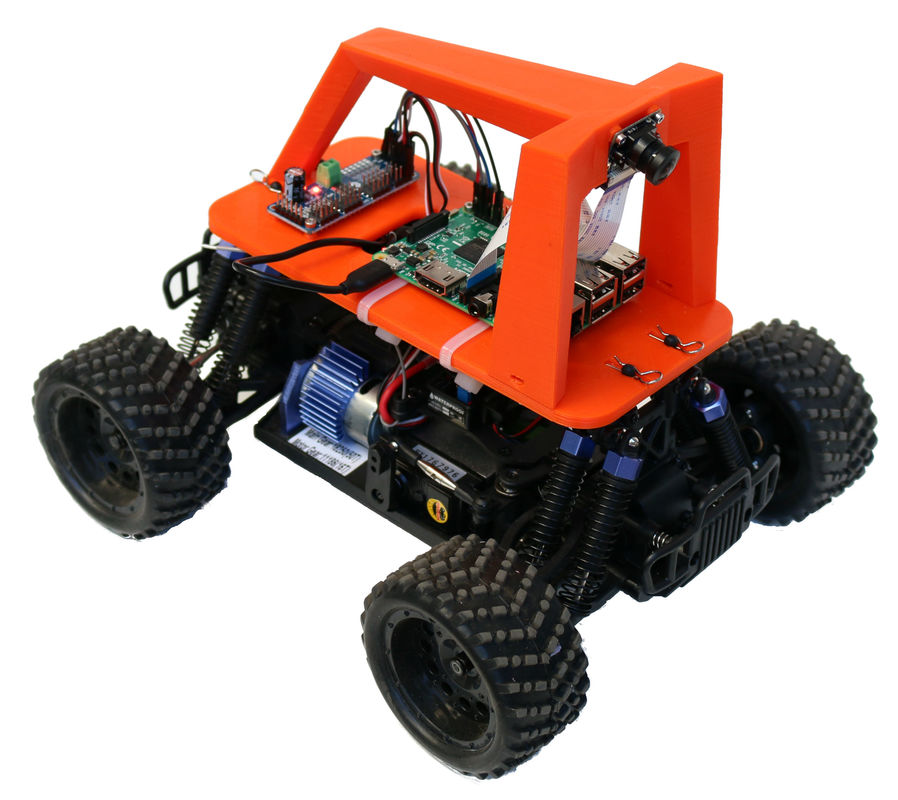
\includegraphics[scale=0.2]{img/donkey.jpg}
\caption{Example of a ``DonkeyCar'', an opensource DIY self driving small car}
\end{figure}

In addition, it's good to know that both thermal motors and cloud computation\footnote{During the race only, training of the model can be done on the cloud} are forbiddens and that the total budget cannot exceed 500\euro{}.

\subsection{Start and Finish}
The car have to be able to start the race by itself after a luminous countdown done by a traffic light of 10x10cm (red, yellow and green). If the car has not start 2 mn after the start, it will be discalified. Each vehicle has the right to a false start, after it will be penalysed. \\

The same way, the vehicule must be able to stop itself maximum 5s after crossing the finish line. This line will be yellow and 15cm long accross the wole width.\\

Any breaches of these rules will result in a penalty:
\begin{itemize}
\item 5s for a false start (after the autorized one)
\item 5s if the car hasn't stop itself in the 5s limits
\end{itemize}

\subsection{Circuit}
The circuit will be made of 2cm wide white marking on top of a 4cm wide black marking on each side of the lane, and will be 45 meters long. Obstacle of 10x10x10cm will be set on the track and could change between each race. The speed is limited to 65km/h.\footnote{Even though it's pretty unlikely that any car can reach this speed in autonomous mode.}\\
So the car must be able to identify those lane and drive without crossing them.\\

\begin{figure}[!h]
\centering
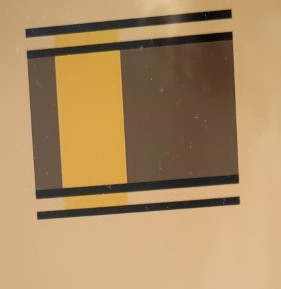
\includegraphics[angle=-90,width=10cm]{img/road.jpeg}
\caption{Representation of the Finish line}
\end{figure}
\clearpage

